\documentclass[11pt, oneside]{article}   	% use "amsart" instead of "article" for AMSLaTeX format
\usepackage{geometry}                		% See geometry.pdf to learn the layout options. There are lots.
\geometry{letterpaper}                   		% ... or a4paper or a5paper or ... 
%\geometry{landscape}                		% Activate for for rotated page geometry
%\usepackage[parfill]{parskip}    		% Activate to begin paragraphs with an empty line rather than an indent
\usepackage{graphicx}				% Use pdf, png, jpg, or eps§ with pdflatex; use eps in DVI mode
\usepackage{amsmath}
\usepackage{amssymb}
\setlength\parindent{0pt}

\usepackage{caption} 
\usepackage{float}
\usepackage{hyperref}
	\hypersetup{
    colorlinks=true,
    linkcolor=blue,
    filecolor=blue,      
    urlcolor=blue,
}
\usepackage{tikz}				% Use pdf, png, jpg, or eps§ with pdflatex; use eps in DVI mode
\usetikzlibrary{decorations.pathreplacing,positioning, arrows.meta}

 \date{} 

\title{On balance tests}

\begin{document}
\maketitle
%\section{}
%\subsection{}
Let  $Y_i $ be a continuous (or discrete) variable and  $ T_i $ a dummy variable which takes either values one or zero with probability $p$ and $1-p$, respectively. A regression of $Y_i $ on $T_i$ and a constant is equivalent to comparing means for the two groups (one with values of $T=0$ and the other with values of $T=1$). It can be shown that:


 \begin{align*}
	\beta = \frac{cov[Y, T]}{var(T)}=\frac{p(1-p)(E[Y_i|T_i=1]- E[Y_i|T_i=0])}{p(1-p)}=E[Y_i|T_i=1]- E[Y_i|T_i=0]
 \end{align*}

In case of endogenous regressor, mean comparison and linear regression suffer from the same bias. To see this:

 \begin{align*}
 	E[Y_i|T_i=1] &=&  \alpha +  \beta  +  E[\varepsilon_i|T_i=1] \\
 	E[Y_i|T_i=0] &=&  \alpha  + E[\varepsilon_i|T_i=0]\\
 	E[Y_i|T_i=1]- E[Y_i|T_i=0] &= &  \beta +  \underset{\text{selection bias}}{\underbrace{ E[\varepsilon_i|T_i=1] -   E[\varepsilon_i|T_i=0] }}
 \end{align*}
 
\newpage

 A numerical example is shown in Table \ref{t: selection}. Each column denotes a different relationship between $Y$ on $T$. In the top part of the table, the row corresponding to $T$, depicts coefficient estimate (and standard error in parenthesis) from a regression of $Y$ on $T$.  In the bottom part of the table the mean difference between the two groups, namely those with $T=1$ and $T=0$, as well as the corresponding standard error are shown. 
 Try it for yourself, the replication material is on  \href{https://github.com/CEU-Economics-and-Business/ECBS6233-Empirical-Research/tree/master/code}{GitHub}.

\begin{table} [H]
\begin{center}
 
 \caption{Comparisons of means \label{t: selection}}

\begin{tabular}{l*{3}{c}}
\hline\hline
                    &\multicolumn{3}{c}{}                  \\
                    &\multicolumn{1}{c}{(1)}&\multicolumn{1}{c}{(2)}&\multicolumn{1}{c}{(3)}\\
\hline
T                   &       0.699&       0.740&       0.696\\
                    &     (0.013)&     (0.024)&     (0.020)\\
\hline
Mean-Difference     &       0.699&       0.740&       0.696\\
Standard Error      &       0.013&       0.024&       0.020\\
\hline\hline
\end{tabular}


\linespread{1.5}
\vspace{0.1cm}
\par
\begin{minipage}{0.8\linewidth}
\baselineskip10pt
{\scriptsize {Notes:  The relationship between Y and T is $ Y=0.5+ 0.7 \cdot T+ \varepsilon $ in column (1), $ Y=0.5+ 0.7 \cdot T+0.3* X_1 + \varepsilon $ in column (2), and in column (3) $ Y=0.5+ 0.7 \cdot T+0.15* X_2 + \varepsilon $ where $X_2$ is itself a linear function of $X_1$.}}
\end{minipage}
\end{center}
\end{table}

\newpage

A covariate balance test helps us understand if treatment and control group are actually comparable. The variables to include in a balancing test are usually measured pre-treatment. See Figure  \ref{fig:tikz} for a visual representation. Geographical variables such as latitude, longitude, altitude, ruggedness, distance, surface are also unlikely to be affected by the treatment and can be included in a balance test. \\


\begin{figure}[H]
\caption{\label{fig:tikz} Timeline treatment }

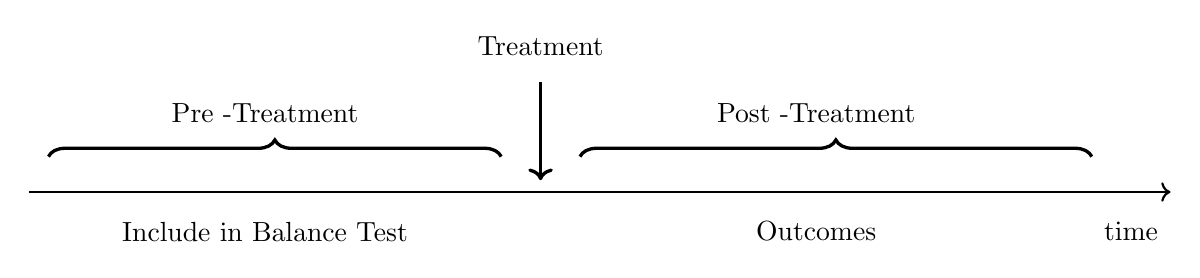
\begin{tikzpicture}

\draw [thick,->] (0,0) -- (14.5,0);
\node[align=left] at (14,-0.5) {time};

\node[align=center] at (3,1) {Pre -Treatment};
\draw [very thick, decorate,decoration={brace,amplitude=6pt,raise=0pt}] (0.25,0.45) -- (6,0.45);
\node[align=center] at (3,-0.5) {Include in Balance Test};

\node[align=center] at (6.5,1.85) {Treatment};
\draw [very thick,->] (6.5,1.4) -- (6.5,0.15);

\node[align=center] at (10,1) {Post -Treatment};
\draw [very thick, decorate,decoration={brace,amplitude=6pt,raise=0pt}] (7,0.45) -- (13.50,0.45);
\node[align=center] at (10,-0.5) {Outcomes};

\end{tikzpicture}
\end{figure}


If the variables are measured post-treatment, it's likely they are affected by the treatment, therefore they should not be included in a balancing test; they are outcomes. \\

We encourage you to use visual representations to show covariate balance if possible. A nice example of pre and post mean comparison is shown in Figure \ref{fig:aej} where raw means are plotted before and after treatment. An alternative way is showing coefficient plots. Feel free to experiment alternative options and be creative.

\begin{figure} [H]
\begin{center}
\caption{\label{fig:aej} Incentives, commitments, and habit formation}
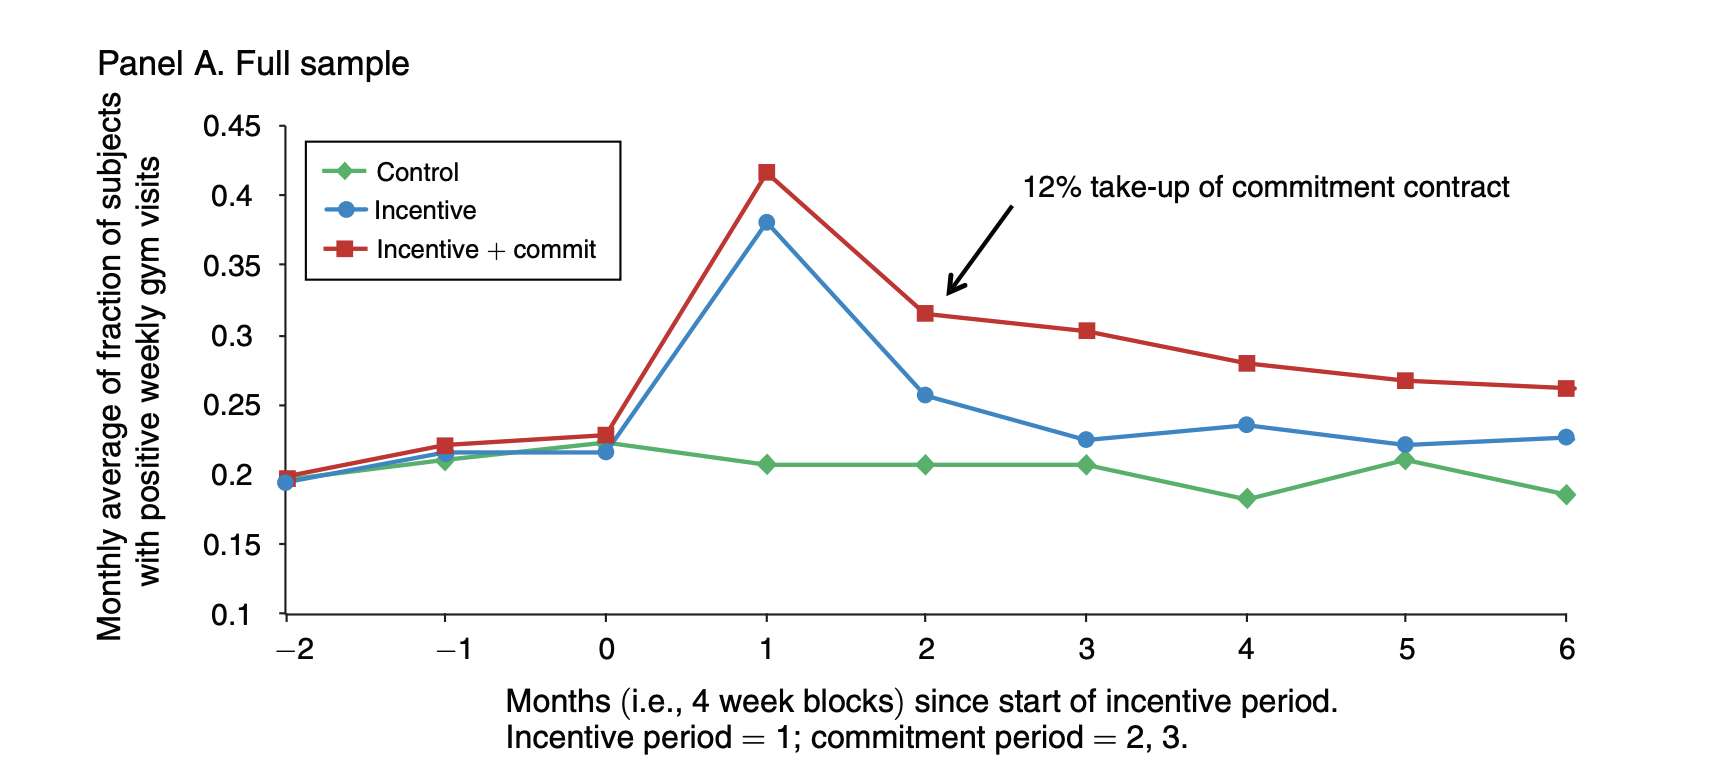
\includegraphics[width=120 mm, height=60 mm]{output/figures/Habit_Formation_Exercise.png} 
\end{center}
\vspace{0.1cm}
\par
\begin{minipage}{ \linewidth}
\baselineskip10pt
\scriptsize{Notes: Figure from Royer, Heather, Mark Stehr, and Justin Sydnor. "Incentives, commitments, and habit formation in exercise: evidence from a field experiment with workers at a fortune-500 company." American Economic Journal: Applied Economics 7.3 (2015): 51-84.}
\end{minipage}
\end{figure}





In many cases, it makes sense to have a mean comparison controlling for other factors. For example, if the assignment is stratified, you would want to look at the regression coefficient once you have controlled for other factors i.e include school fixed effects, $ \eta_s $, because the treatment is stratified at the school level.  $\rho$ is the parameter of interest.


\begin{align*}
x_i =  \alpha + \rho T_i + \eta_s + \varepsilon_i
\end{align*}
 
 
 If you are testing if one, or several covariates, are affecting treatment, straightforward tests are bivariate regressions of the form:
 
 \begin{align*}
T_i = \alpha + \beta x_i+ \varepsilon_i
\end{align*}
 
The $\beta$ coefficients inform us if one or some covariates affect treatment individually.\\


In case you want to check whether several variables affect the treatment  jointly, the specification to run is:
 \begin{align*}
 T_i = \alpha + X_i ^\intercal \gamma+ \eta_s + \varepsilon_i
\end{align*}
 
Note that $X_i$ is a vector of covariates. An $F$-test on the joint significance, whether all covariates jointly affect treatment, should be reported.


\end{document}  